% ===========================================================================
% Construire des arbres de décision
% Traduit et adapté de :
%   https://www.bootstrapworld.org/materials/fall2026/en-us/lessons/decision-trees-building/
% Adapté au contexte français (noms de colonnes et espèces en français)
% Licence : Creative Commons 4.0 Unported (Bootstrap Community)
% ===========================================================================

\documentclass[12pt,a4paper]{article}

% ---------- Packages ----------
\usepackage[utf8]{inputenc}
\usepackage[T1]{fontenc}
\usepackage{libertine}
\usepackage{microtype}
\usepackage[french]{babel}
\usepackage{graphicx}
\usepackage{float}
\usepackage{hyperref}
\usepackage{geometry}
\usepackage{enumitem}
\usepackage{tabularx}
\usepackage{xcolor}
\usepackage[raster]{tcolorbox}
\usepackage{booktabs}
\usepackage{fancyhdr}
\usepackage{titlesec}
\usepackage{amsmath}
\usepackage{amssymb}
\usepackage{listings}
\usepackage{tikz}
\usetikzlibrary{trees, arrows.meta, positioning, shapes.geometric, calc}

% ---------- Mise en page ----------
\geometry{margin=2.5cm, headheight=15pt, footskip=30pt}
\fancyhf{}
\fancyhead[L]{\textbf{Construire des arbres de décision}}
\fancyhead[R]{\thepage}
\fancyfoot[C]{Bootstrap Community — CC BY 4.0}
\renewcommand{\headrulewidth}{0.4pt}
\pagestyle{fancy}

% ---------- Couleurs ----------
\definecolor{bsblue}{RGB}{41,128,185}
\definecolor{bsgreen}{RGB}{39,174,96}
\definecolor{bsorange}{RGB}{230,126,34}
\definecolor{bsgray}{RGB}{149,165,166}
\definecolor{codebg}{RGB}{245,247,250}
\definecolor{leafgreen}{RGB}{39,174,96}
\definecolor{nodeorange}{RGB}{230,126,34}
\definecolor{rootblue}{RGB}{41,128,185}

% ---------- Styles de sections ----------
\titleformat{\section}[hang]{\Huge\bfseries\color{bsblue}}{}{0pt}{}[\vspace{-0.5em}\rule{\textwidth}{2pt}]
\titleformat{\subsection}[hang]{\Large\bfseries\color{bsblue!80!black}}{}{0pt}{}
\titleformat{\subsubsection}[hang]{\large\bfseries\color{bsgreen!60!black}}{}{0pt}{}

% ---------- Environnements personnalisés ----------
\newtcolorbox{overviewbox}{
  colback=bsblue!5!white, colframe=bsblue!60!white,
  fonttitle=\bfseries, title=Objectif de la section,
  left=1em, right=1em, top=0.5em, bottom=0.5em
}
\newtcolorbox{activitybox}{
  colback=bsgreen!5!white, colframe=bsgreen!60!white,
  fonttitle=\bfseries, title=Activité,
  left=1em, right=1em, top=0.5em, bottom=0.5em
}
\newtcolorbox{thinkbox}{
  colback=bsorange!5!white, colframe=bsorange!60!white,
  fonttitle=\bfseries, title=Réflexion,
  left=1em, right=1em, top=0.5em, bottom=0.5em
}
\newtcolorbox{keypointbox}{
  colback=bsgray!10!white, colframe=bsgray!50!white,
  fonttitle=\bfseries, title=Point clé,
  left=1em, right=1em, top=0.5em, bottom=0.5em
}
\newtcolorbox{instructornotes}{
  colback=yellow!10!white, colframe=yellow!80!black,
  fonttitle=\bfseries, title=Notes pour l'enseignant·e,
  left=1em, right=1em, top=0.5em, bottom=0.5em
}
\newtcolorbox{codebox}{
  colback=codebg, colframe=bsgray!40,
  fonttitle=\bfseries, title=Code Pyret,
  left=1em, right=1em, top=0.5em, bottom=0.5em
}
\newtcolorbox{contractbox}{
  colback=bsblue!3!white, colframe=bsblue!40!white,
  left=1em, right=1em, top=0.6em, bottom=0.6em
}

% ---------- Style listings pour Pyret ----------
\lstdefinelanguage{Pyret}{
  keywords={use,context,url-file,and,or,not,if,else,for,fun,data,sharing,include,import,as,where,let,rec,is,=,true,false,load-table,source,end,Row,String,Number,Boolean,Table,Image},
  sensitive=true,
  comment=[l]{\#},
  morestring=[b]",
  morestring=[b]',
}
\lstset{
  language=Pyret,
  basicstyle=\ttfamily\small,
  commentstyle=\color{bsgreen!70!black}\itshape,
  keywordstyle=\color{bsblue}\bfseries,
  stringstyle=\color{bsorange},
  backgroundcolor=\color{codebg},
  frame=single,
  framesep=5pt,
  rulecolor=\color{bsgray!40},
  breaklines=true,
  breakatwhitespace=false,
  showstringspaces=false,
  aboveskip=0.8em,
  belowskip=0.8em,
}

% ---------- Commandes pratiques ----------
\newcommand{\img}[3]{%
  \begin{figure}[H]
    \centering
    \includegraphics[#2]{#1}
    \caption{#3}
    \label{fig:#1}
  \end{figure}
}
\newcommand{\contrat}[1]{%
  \begin{contractbox}
    \ttfamily #1
  \end{contractbox}
}

% ---------- Arbre de décision TikZ ----------
% Styles prédéfinis pour les arbres de décision : noeud racine, noeud de
% décision, noeud feuille, et arêtes étiquetées oui/non.
\tikzset{
  root/.style={draw=rootblue, thick, fill=rootblue!15, rounded corners=4pt,
               align=center, font=\small\bfseries, text=rootblue, inner sep=4pt, minimum width=2.5cm},
  decision/.style={draw=nodeorange, thick, fill=nodeorange!10, rounded corners=4pt,
                   align=center, font=\small\bfseries, text=nodeorange!80!black, inner sep=4pt, minimum width=2.5cm},
  leaf/.style={draw=leafgreen, thick, fill=leafgreen!10, rounded corners=4pt,
               align=center, font=\small\bfseries, text=leafgreen!70!black, inner sep=4pt, minimum width=2.5cm},
  split-yes/.style={->, >=Stealth, thick, draw=bsgreen, font=\scriptsize\bfseries},
  split-no/.style={->, >=Stealth, thick, draw=bsorange, font=\scriptsize\bfseries},
}

% ---------- Informations du document ----------
\title{%
  \vspace{-2cm}
  {\Huge\bfseries Construire des}\\[0.3em]
  {\Huge\bfseries arbres de décision}\\[0.5em]
  {\large Classificateurs, if-then-else, et apprentissage supervisé}\\[1em]
  {\normalsize Traduit et adapté depuis \href{https://www.bootstrapworld.org/materials/fall2026/en-us/lessons/decision-trees-building/}{Bootstrap World} (Fall 2026)}\\
  {\normalsize Adapté au contexte francophone — colonnes et espèces en français}\\[0.5em]
  {\normalsize Licence Creative Commons 4.0 International}
}
\date{}
\author{}

\begin{document}

\maketitle
\thispagestyle{empty}

\vspace{2cm}
\begin{center}
  \textit{Ces supports ont été développés en partie grâce au soutien de la National Science Foundation\\
  (bourses 1042210, 1535276, 1648684, 1738598, 2031479 et 1501927).}
\end{center}

\newpage
\tableofcontents
\newpage

% ===========================================================================
% SECTION 1 : PRÉDIRE DES CATÉGORIES
% ===========================================================================
\section{Prédire des catégories}

\begin{overviewbox}
  Les élèves découvrent les \emph{classificateurs} et construisent des \textbf{arbres de décision} en jouant à une version adaptée du jeu «~Je vois, je vois~». Ils apprennent ce qu'est un arbre de décision, qu'il existe plusieurs arbres possibles pour un même jeu de données, et que la qualité d'un arbre dépend de la façon dont it sépare les données.
\end{overviewbox}

% ---------- Launch ----------
\subsection{Lancement}

Considérez chacune des trois situations suivantes~:

\begin{itemize}
  \item Vous et vos ami·es passez un quiz en ligne qui tente de deviner votre coiffure.
  \item Deux personnes qui travaillent pour la \emph{même entreprise} et gagnent le \emph{même salaire} demandent un prêt à la banque en remplissant le \emph{même formulaire en ligne}. L'une obtient le prêt, l'autre non.
  \item Un·e journaliste affiche une carte avec certains États colorés en bleu et d'autres en rouge. Iel explique que les prédictions de la carte pour l'élection à venir ont été établies à partir de données historiques du recensement.
  \item Une caméra à la banque prend une photo de votre visage, dans l'espoir de la faire correspondre à votre identité.
\end{itemize}

\begin{thinkbox}
  \textbf{Qu'est-ce que tous ces exemples ont en commun~?}

  En surface, ces situations ne semblent pas avoir grand-chose en commun. Mais tous sont des exemples de \textbf{classificateurs} — une sorte de fonction qui~:
  \begin{enumerate}
    \item reçoit une entrée~;
    \item pose des questions sur cette entrée~;
    \item utilise les réponses pour produire un résultat prédit à partir d'une liste de catégories.
  \end{enumerate}
\end{thinkbox}

\begin{thinkbox}
  \begin{itemize}
    \item Quelles données pensez-vous être utilisées pour \textbf{deviner votre coiffure}~?
    \begin{itemize}
      \item Historique de visionnage, recherches, abonnements aux chaînes, likes, dislikes, activité Google, retours «~non intéressé~».
    \end{itemize}
    \item Quelles données pour \textbf{l'approbation d'un prêt}~?
    \begin{itemize}
      \item Dettes, actifs, historique de paiement, nombre de comptes ouverts, comptes en retard, revenus, charges, découverts des 90 derniers jours.
    \end{itemize}
    \item Quelles données pour \textbf{prédire une élection}~?
    \begin{itemize}
      \item Données du recensement incluant race, genre, niveau de revenu, affiliation politique, âge des votant·es, ainsi que les résultats des années précédentes.
    \end{itemize}
  \end{itemize}
\end{thinkbox}

\begin{keypointbox}
  Les classificateurs sont des fonctions qui associent une entrée à un ensemble possible de cibles.

  \vspace{0.5em}
  \begin{center}
  \begin{tabularx}{\textwidth}{l X X}
    \toprule
    \textbf{Exemple} & \textbf{Données d'entrée (connues)} & \textbf{Catégories (inconnues)} \\
    \midrule
    Quiz coiffure    & Sexe, âge, race, musique, code postal…       & Queue de cheval vs. coupe courte vs. dreadlocks vs. crew cut vs. mohawk… \\
    Prêt bancaire     & Revenu, emploi, âge, score de crédit…         & Approuvé vs. Non approuvé \\
    Élections         & Votes passés, sondages récents…              & Bleu vs. Rouge \\
    Reconnaissance faciale & Votre visage                            & Toute personne enregistrée \\
    \bottomrule
  \end{tabularx}
  \end{center}

  \vspace{0.5em}
  Par exemple, le quiz de coiffure \emph{probablement} éliminera «~queue de cheval~» si la personne qui le passe est «~masculine~», mais il ne se trompera pas toujours~: après tout, certain·es hommes portent une queue de cheval~! Le travail d'un classificateur est de deviner l'\textbf{option la plus probable} à partir des données d'entraînement.

  \vspace{0.5em}
  \emph{La plupart des modèles se trompent. Certains sont utiles.}
\end{keypointbox}

% ---------- Investigate: I Spy Classify ----------
\subsection{Exploration~: «~Je vois… Classifier~!~»}

Les classificateurs utilisent ce qu'on appelle un \textbf{arbre de décision}~: ils posent des questions pour réduire les résultats possibles jusqu'à atteindre un seul résultat prédit.

Si vous avez déjà joué à «~Je vois, je vois avec mon petit œil~», vous avez déjà construit un arbre de décision~! Les règles sont simples~:
\begin{itemize}
  \item Un·e joueur·euse pense à quelque chose que tout le monde peut voir.
  \item Iel donne un indice~: «~Je vois… quelque chose de bleu~!~»
  \item Les autres joueur·euses posent des questions fermées (oui/non) pour deviner.
\end{itemize}

\begin{activitybox}
  Nous allons jouer à une version «~Je vois… \textbf{Classifier}~!~»~:
  \begin{itemize}
    \item Tout le monde se lève à sa place.
    \item L'enseignant·e choisit un·e élève comme cible, sans le dire à personne.
    \item Tour à tour, les élèves posent des questions fermées.
    \item Vous pouvez poser des questions \emph{catégorielles}~: «~porte-t-iel des lunettes~?~»
    \begin{itemize}
      \item Si la réponse est «~oui~», seul·es les élèves portant des lunettes restent debout.
      \item Si la réponse est «~non~», seul·es ceux·celles qui \emph{ne portent pas} de lunettes restent.
    \end{itemize}
    \item Vous pouvez poser des questions \emph{quantitatives}~: «~mesure-t-iel plus de 1~m~70~?~»
    \begin{itemize}
      \item Si «~oui~», seul·es les élèves de plus de 1~m~70 restent.
      \item Si «~non~», seul·es ceux·celles de 1~m~70 ou moins restent.
    \end{itemize}
  \end{itemize}
\end{activitybox}

\img{images/ed6943172cbca1a7.png}{width=0.35\textwidth}{Une partie d'un arbre de décision montrant le nombre d'élèves qui portent ou non des lunettes.}

\begin{instructornotes}
  Pendant que la classe essaie de deviner la cible, dessinez au tableau la progression sous forme d'organigramme, avec des arêtes «~oui~» et «~non~» ramifiées vers la gauche et la droite. Sur chaque arête, notez le nombre d'élèves pour qui la réponse est «~oui~» et «~non~». Continuez jusqu'à ce que la classe ait trouvé la cible.
\end{instructornotes}

\img{images/457300360bb30eee.png}{width=0.4\textwidth}{Un arbre de décision représentant la recherche d'un·e élève en classe, montrant les nombres d'élèves qui portent ou non des lunettes, qui ont ou non les cheveux roux, et qui sont ou non des filles. Ici, la cible identifiée est «~Jimmy~».}

\begin{thinkbox}
  \begin{itemize}
    \item \textbf{Combien de questions} a-t-il fallu pour trouver la cible~?
    \item \textbf{Si vous aviez posé «~s'appelle-t-iel XYZ~?~» en boucle jusqu'à trouver la cible~?} Auriez-vous fini par trouver~?
    \begin{itemize}
      \item Oui, mais cela aurait pris \emph{beaucoup plus longtemps}~! Poser des questions sur des groupes a permis d'éliminer des cibles possibles et de réduire les choix plus rapidement.
    \end{itemize}
  \end{itemize}
\end{thinkbox}

\begin{activitybox}
  Rejouons quelques manches. Cette fois, cependant, nous ne pouvons \emph{qu'ajouter} à notre arbre~: pour tout le reste, il faut poser les mêmes questions dans le même ordre.
\end{activitybox}

\begin{instructornotes}
  Rejouez quelques manches. Essayez de choisir des élèves qui forceront la classe à \textbf{ajouter à leur arbre}. Pour chaque élève classifié, demandez à la classe combien de questions ont été nécessaires.

  Encouragez-les à poser un mélange de questions catégorielles et quantitatives. Si les élèves commencent à se plaindre d'être «~coincé·es~» avec leurs premières questions, c'est bon signe~! Demandez-leur ce qu'ils changeraient et pourquoi — un excellent moyen de faire émerger leur intuition sur ce qui fait un «~bon~» arbre de décision.
\end{instructornotes}

\begin{center}
  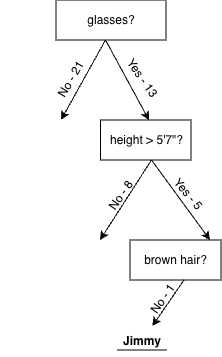
\includegraphics[height=4cm]{images/457300360bb30eee.png}\hspace{1.5em}
  
\includegraphics[height=1.2cm]{images/39a531d92bbe1cfd.png}\hspace{1.5em}
  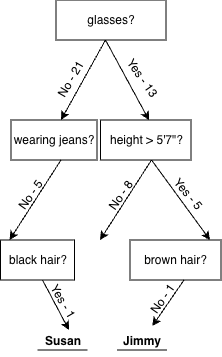
\includegraphics[height=4cm]{images/d608631a49759afa.png}
\end{center}

\begin{thinkbox}
  \begin{itemize}
    \item Dans ce jeu, quelles étaient nos «~cibles~»~?
    \begin{itemize}
      \item Les élèves de la classe.
    \end{itemize}
    \item Combien de cibles possibles avions-nous~?
    \begin{itemize}
      \item Le nombre d'élèves dans la classe.
    \end{itemize}
    \item Si vous pouviez recommencer, comment changeriez-vous cet arbre de décision~?
    \begin{itemize}
      \item Grande question~! Laissez les élèves discuter.
    \end{itemize}
    \item Si notre première question était «~porte-t-iel des lunettes~?~» et qu'un seul élève porte des lunettes~: si cet élève est la cible, combien de questions supplémentaires seront nécessaires~?
    \begin{itemize}
      \item Aucune~! Si la réponse est «~oui~», on sait immédiatement qui c'est.
    \end{itemize}
    \item Serait-ce la \emph{meilleure} première question si on devait jouer souvent~?
    \begin{itemize}
      \item Non, car si la réponse est «~non~» on n'a pas réduit grand chose.
    \end{itemize}
    \item Si \emph{presque tous} les élèves mesurent 1~m~70 ou plus, «~mesure-t-iel plus de 1~m~70~?~» serait-il une bonne première question~?
    \begin{itemize}
      \item Non, car la question ne sépare pas le groupe d'une façon qui reflète la variation réelle des données.
    \end{itemize}
    \item Quand est-ce que «~plus de 1~m~70~?~» serait une \emph{bonne} question~?
    \begin{itemize}
      \item Si elle divise la classe aussi près que possible «~en deux~».
    \end{itemize}
  \end{itemize}
\end{thinkbox}

% ---------- Decision Tree Terminology ----------
\subsubsection{Vocabulaire des arbres de décision}

\img{images/240cc53427b98982.png}{width=0.5\textwidth}{Un arbre de décision utilisé pour introduire le vocabulaire~: nœud, nœud racine, nœud feuille.}

\begin{keypointbox}
  \textbf{Vocabulaire des arbres de décision}
  \begin{itemize}
    \item Un \textbf{nœud de décision} (\emph{decision node}) divise un jeu de données selon les valeurs d'une de ses colonnes. C'est une «~question~».
    \item Le tout premier nœud (en haut) est appelé le \textbf{nœud racine} (\emph{root node}). Il représente le jeu de données entier.
    \item Chaque division crée davantage de branches et de nœuds, représentant des sous-ensembles de données selon une nouvelle «~question~» sur une colonne.
    \item Un \textbf{nœud feuille} (\emph{leaf node}) contient le résultat prédit, et n'a pas d'autres branches. Les résultats proviennent d'une colonne désignée du jeu de données.
  \end{itemize}
\end{keypointbox}

\begin{instructornotes}
  Nous nous limitons aux divisions qui ne créent que deux branches, mais certains arbres de décision utilisent des divisions en 3, 10 ou plus. Les informaticien·nes appellent la séquence de questions depuis la racine jusqu'à un résultat un «~chemin~» (\emph{path}).

  Discutez de l'arbre de décision construit pendant le jeu pour aider les élèves à identifier le nœud racine, les nœuds de décision, les nœuds feuilles et les chemins.
\end{instructornotes}

% ---------- Investigate: Animals Dataset ----------
\subsection{Exploration~: le jeu de données des animaux}

Nous allons jouer à une autre manche de «~Je vois… Classifier~!~», mais cette fois avec un vrai jeu de données d'animaux.

\begin{center}
\begin{tabularx}{\textwidth}{l l l r l l l}
  \toprule
  \textbf{nom} & \textbf{espece} & \textbf{sexe} & \textbf{poids} & \textbf{queue} & \textbf{mammifere} & \textbf{nage} \\
  \midrule
  Firepaw    & chat      & male      & 9.50  & TRUE  & TRUE  & FALSE \\
  Leafpool   & chat      & femelle   & 10.60 & TRUE  & TRUE  & FALSE \\
  Shadestar  & chat      & femelle   & 9.00  & TRUE  & TRUE  & TRUE  \\
  Bramble    & chat      & femelle   & 4.10  & TRUE  & TRUE  & FALSE \\
  Brick      & chat      & male      & 8.50  & TRUE  & TRUE  & FALSE \\
  Frisky     & chien     & femelle   & 9.60  & TRUE  & TRUE  & TRUE  \\
  Socks      & chien     & femelle   & 10.00 & TRUE  & TRUE  & TRUE  \\
  Stripe     & chien     & male      & 11.10 & TRUE  & TRUE  & TRUE  \\
  Snickers   & chien     & male      & 10.30 & TRUE  & TRUE  & TRUE  \\
  Bruni      & lezard    & femelle   & 8.20  & TRUE  & FALSE & TRUE  \\
  Jesús      & lezard    & male      & 3.50  & TRUE  & FALSE & FALSE \\
  Gary       & escargot  & hermaphrodite & 0.02  & FALSE & FALSE & FALSE \\
  Turbo      & escargot  & hermaphrodite & 0.03  & FALSE & FALSE & FALSE \\
  Charlotte  & tarentule & male      & 0.35  & FALSE & FALSE & FALSE \\
  Webs       & tarentule & femelle   & 0.40  & FALSE & FALSE & FALSE \\
  \bottomrule
\end{tabularx}
\end{center}

\begin{thinkbox}
  \begin{itemize}
    \item Que \textbf{remarquez}-vous sur les animaux dans ce jeu de données~?
    \begin{itemize}
      \item Les réponses varieront~: Shadestar est un chat qui nage~!~Charlotte est une tarentule mâle~!~Les escargots sont très légers~!
    \end{itemize}
    \item Quels \textbf{types de données} voyez-vous dans cette table~?
    \begin{itemize}
      \item Strings (\texttt{nom}, \texttt{espece}, \texttt{sexe}), Numbers (\texttt{poids}), Booleans (\texttt{queue}, \texttt{mammifere}, \texttt{nage}).
    \end{itemize}
  \end{itemize}
\end{thinkbox}

\begin{keypointbox}
  Un arbre de décision est une façon de \textbf{modéliser la structure cachée} dans les données.

  Contrairement aux humains, qui peuvent inventer leurs propres questions, les algorithmes d'apprentissage automatique \emph{génèrent} des arbres de décision à partir de jeux de données d'entraînement, en utilisant les en-têtes de colonnes comme questions. Chaque nœud dans l'arbre divise le jeu de données, nous permettant de faire la meilleure prédiction possible sur un résultat.

  Construire un arbre de décision est une forme d'\textbf{apprentissage supervisé}, car les données d'entraînement contiennent déjà les résultats souhaités (dans une colonne), et l'algorithme apprend une fonction qui fait correspondre les entrées aux résultats.
\end{keypointbox}

\begin{activitybox}
  \begin{itemize}
    \item L'enseignant·e choisit un animal du jeu de données.
    \item Votre travail est de deviner son \emph{espèce} (chat, chien, lézard, escargot, ou tarentule).
    \item Vous pouvez poser toutes les questions qui peuvent être répondues en utilisant les colonnes de la table.
  \end{itemize}

  En petits groupes, jouez quelques manches~! Certaines questions sont-elles meilleures que d'autres~?

  Au mur ou sur une feuille de brouillon~: quel est, selon vous, le \textbf{meilleur nœud racine} pour ce jeu de données~? (C'est-à-dire~: quelle est la question la plus utile pour commencer~?) Pouvez-vous expliquer pourquoi vous avez choisi cette question~?
\end{activitybox}

\begin{instructornotes}
  Encouragez les élèves à proposer à la fois des questions catégorielles et quantitatives, et demandez-leur sans cesse d'expliquer \emph{pourquoi} ils ont choisi cette division.

  Pendant qu'iels explorent, dessinez l'arbre de décision au fur et à mesure. Le format Desmos «~Choosing a Root Node~» peut accompagner cette exploration.
\end{instructornotes}

% ---------- Synthesize ----------
\subsection{Synthèse}

\begin{thinkbox}
  \begin{itemize}
    \item En quoi \emph{générer des questions} à partir d'un jeu de données était-il \emph{similaire} au jeu «~Je vois… Classifier~!~» précédent~?
    \begin{itemize}
      \item Certaines questions faisaient un meilleur travail de séparation des données que d'autres.
    \end{itemize}
    \item En quoi était-ce \emph{différent}~?
    \begin{itemize}
      \item Il y avait des questions que nous ne pouvions pas poser, car il n'y avait pas de colonne pour elles~!
    \end{itemize}
  \end{itemize}
\end{thinkbox}

\begin{keypointbox}
  Vous avez appris que certains arbres de décision sont meilleurs que d'autres. Par exemple, la \emph{fréquence de chaque catégorie} affecte le «~meilleur nœud~» («~si tout le monde porte des lunettes…~»).

  Lors du choix d'une division pour notre nœud racine, notre but est de poser une question qui sépare les données en \emph{tas les plus nets et organisés possibles}. Par exemple, il serait idéal d'avoir tous les chats d'un côté et tous les chiens de l'autre. Nous ne pouvons pas toujours obtenir une séparation parfaite, mais nous voulons nous en approcher autant que possible.
\end{keypointbox}

\begin{thinkbox}
  \begin{itemize}
    \item \textbf{Comment sait-on qu'une question est bonne pour commencer~?}
    \begin{itemize}
      \item Les bonnes questions aident à éliminer beaucoup de catégories restantes, que la réponse soit oui \emph{ou} non.
    \end{itemize}
    \item \textbf{Que voulons-nous être vrai pour chaque question que nous posons~?}
    \begin{itemize}
      \item Qu'elle sépare la liste des cibles possibles le plus proprement possible, tout en éliminant autant d'options que possible.
    \end{itemize}
    \item \textbf{Comment utilise-t-on un arbre de décision pour faire des prédictions~?}
    \begin{itemize}
      \item On pose la question à la racine de l'arbre, puis on suit les branches pour poser des questions supplémentaires jusqu'à atteindre une catégorie à la fin d'un chemin.
    \end{itemize}
    \item Si nous jouions à «~Classifier~», mais en devinant quel \textbf{pays} je pense~: quelle serait une bonne première question~?
    \begin{itemize}
      \item Est-ce un pays de l'hémisphère occidental~?
      \item Est-ce un pays où l'on parle espagnol~?
    \end{itemize}
  \end{itemize}
\end{thinkbox}

\newpage

% ===========================================================================
% SECTION 2 : CONSTRUIRE DES ARBRES DE DÉCISION EN PYRET
% ===========================================================================
\section{Construire des arbres de décision en Pyret}

\begin{overviewbox}
  Les élèves apprennent à écrire une fonction \emph{classificateur} en Pyret pour prédire l'espèce d'un animal, en utilisant des expressions \texttt{if/else} pour poser des questions sur une ligne (\emph{row}) de la table. Ils utilisent \texttt{image-dot-plot} et \texttt{classify} pour visualiser et évaluer leur arbre.
\end{overviewbox}

% ---------- Launch ----------
\subsection{Lancement}

Apprenons à écrire une fonction classificateur pour prédire l'espèce en Pyret~!

\begin{keypointbox}
  Rappelez-vous~:
  \begin{itemize}
    \item Une fonction consomme une entrée et produit une sortie.
    \item Pour la \emph{même entrée}, une fonction doit produire le \emph{même résultat} — à chaque fois.
    \item Cela signifie que les classificateurs sont \emph{juste des fonctions~!} Notre classificateur classera le même animal de la même façon, à chaque fois.
    \begin{itemize}
      \item S'il prédit que \texttt{firepaw} est un chat, il prédira \emph{toujours} cela.
      \item S'il prédit que \texttt{firepaw} est un escargot, il prédira \emph{toujours} cela.
    \end{itemize}
  \end{itemize}
\end{keypointbox}

Nous devrons choisir une question, puis écrire une règle.

\img{images/ef358f5d1af925f9.png}{width=0.5\textwidth}{Un arbre de décision représentant une recherche d'espèce d'animal. Le nœud racine divise selon la présence d'une queue. La branche «~non~» contient 2 tarentules et 2 escargots, tandis que la branche «~oui~» contient 2 lézards, 4 chiens et 5 chats.}

\begin{thinkbox}
  Supposons que notre arbre n'ait qu'un seul niveau~: on demande si l'animal a une queue, puis on prend notre meilleure estimation.

  Parmi les 15 animaux de notre jeu de données d'entraînement, 11 ont une queue et 4 n'en ont pas.
  \begin{itemize}
    \item Quelle espèce notre règle devrait-elle prédire pour le côté «~oui~» de l'arbre~?
    \begin{itemize}
      \item «~\texttt{chat}~» — c'est l'espèce la plus commune.
    \end{itemize}
    \item Quelle espèce pour le côté «~non~» de l'arbre~?
    \begin{itemize}
      \item «~\texttt{escargot}~» — escargot et tarentule sont également communs, mais on doit en choisir un.
    \end{itemize}
  \end{itemize}
\end{thinkbox}

\img{images/bc5e602c3d937fd2.png}{width=0.35\textwidth}{Un arbre de décision qui prédit l'espèce d'un animal. Le nœud racine divise selon la présence d'une queue. La branche «~non~» prédit escargot, la branche «~oui~» prédit chat.}

\begin{keypointbox}
  Un arbre de décision est un \textbf{algorithme avec perte} (\emph{lossy algorithm}). Il réduit la complexité et écarte la variance des données, en cherchant des «~règles générales~» qui s'appliquent à \emph{la plupart} — mais pas à la totalité — des données.

  \begin{itemize}
    \item La branche «~oui~» contient plus de chats que toute autre chose (5 sur 11). Même si les chats sont l'espèce la plus probable pour les animaux à queue, notre classificateur ne sera juste qu'environ 45\,\% du temps~!
    \item La branche «~non~» est également répartie entre escargots et tarentules. Quelle que soit l'espèce prédite par notre règle, le classificateur ne sera juste que 50\,\% du temps~!
  \end{itemize}
\end{keypointbox}

\begin{activitybox}
  \begin{itemize}
    \item Ouvrez le \textbf{fichier de démarrage Arbre de Décision} (\texttt{Arbre\allowbreak-Decision\allowbreak-Starter.arr}) et cliquez sur «~Run~».
    \item Remarquez que les premières lignes de la Zone de Définitions chargent les données et définissent 2 tables, appelées \texttt{training} et \texttt{testing}.
    \item Tapez \texttt{training} dans la Zone d'Interactions pour voir la table avec laquelle nous allons travailler pour l'instant.
  \end{itemize}

  Voici comment nous définirions notre \texttt{classifieur-queue} en Pyret~:
\end{activitybox}

\begin{codebox}
\begin{lstlisting}
# classifieur-queue :: Row -> String
# consomme un animal, et predit l'espece
fun classifieur-queue(r):
  if r["queue"] == true:
    "chat"
  else:
    "escargot"
  end
end
\end{lstlisting}
\end{codebox}

\begin{thinkbox}
  Vous avez probablement remarqué que~:
  \begin{itemize}
    \item Comme toute autre fonction, \texttt{classifieur-queue} a un \textbf{contrat}~! Elle consomme une \emph{Row} (un animal) et produit une \emph{String} (l'espèce prédite).
    \item \texttt{classifieur-queue} utilise un \emph{accesseur de ligne} pour accéder à l'information dans la colonne \texttt{"queue"}.
    \item Cette fonction utilise un code que nous n'avons pas vu avant, comme \texttt{if} et \texttt{else}.
  \end{itemize}
\end{thinkbox}

\begin{activitybox}
  \begin{enumerate}[leftmargin=*]
    \item Que fait cette partie de la définition de fonction~?
    \texttt{if r["queue"] == true: "chat"}
    \begin{itemize}
      \item Elle vérifie si la valeur dans la colonne \texttt{"queue"} est \texttt{true}, et si oui, elle classe l'animal comme un «~\texttt{chat}~».
    \end{itemize}
    \item Que fait \texttt{else: "escargot"}~?
    \begin{itemize}
      \item Si la valeur n'est pas \texttt{true}, elle classe l'animal comme un «~\texttt{escargot}~».
    \end{itemize}
    \item Que renvoie \texttt{classifieur-queue(firepaw)}~?
    \begin{itemize}
      \item «~\texttt{chat}~», car Firepaw a une queue.
    \end{itemize}
  \end{enumerate}
\end{activitybox}

\begin{instructornotes}
  Vous trouverez peut-être redondant de vérifier \texttt{r["queue"] == true} puisque la valeur de la cellule est elle-même \texttt{true} ou \texttt{false}~; et vous avez raison~! Le programme fonctionnerait aussi bien en lisant juste \texttt{r["queue"]}. Mais utiliser \texttt{r["queue"] == true} reste cohérent avec la façon dont on utilise les accesseurs de ligne avec les colonnes non booléennes (e.g. \texttt{r["espece"] == "chat"}). L'expérience montre que certain·es élèves s'en sortent mieux si tout reste cohérent.
\end{instructornotes}

% ---------- Investigate: dot plots + classify ----------
\subsection{Visualiser et évaluer l'arbre}

\img{images/18da2d3b592533b5.png}{width=0.55\textwidth}{Un \emph{dot plot} montrant la distribution des valeurs de \texttt{queue} (true/false) sur un petit jeu de données d'animaux. Chaque point est un emoji de l'espèce de l'animal.}

Vous venez de rencontrer deux nouvelles fonctions Pyret qui vont nous aider à donner du sens aux données pendant que nous construisons nos arbres.

\begin{keypointbox}
  \textbf{Deux nouveaux outils}
  \begin{itemize}
    \item La fonction \texttt{image-dot-plot} utilise des emojis pour chaque animal au lieu de points, pour nous aider à voir comment les espèces sont distribuées de part et d'autre de la division de notre classificateur.
    \item La fonction \texttt{classify} ajoute les prédictions de notre classificateur à la table et calcule si elles sont correctes ou non.
  \end{itemize}

  \contrat{\# classify :: (Table t, String colonne-reponse, (Row -> String) classifieur) -> Table}

  \contrat{\# image-dot-plot :: (Table t, String colonne, (Row -> Image) image-fn) -> Image}
\end{keypointbox}

Utilisez l'un de nos nouveaux outils pour répondre aux questions suivantes sur notre arbre \texttt{classifieur-queue}~:

\begin{codebox}
\begin{lstlisting}
image-dot-plot(training, "queue", animal-img)
classify(training, "espece", classifieur-queue)
\end{lstlisting}
\end{codebox}

\begin{thinkbox}
  \begin{itemize}
    \item Pour combien d'animaux \textbf{avec queue} dans le jeu de données d'entraînement, notre arbre à 1 niveau fera-t-il la \emph{bonne} prédiction~?
    \begin{itemize}
      \item 5 — tous les chats.
    \end{itemize}
    \item Pour combien d'animaux \textbf{sans queue}~?
    \begin{itemize}
      \item 2 — tous les escargots.
    \end{itemize}
    \item Pourquoi l'arbre se trompe-t-il pour les chiens et les lézards~?
    \begin{itemize}
      \item Parce qu'iels ont tous une queue, et l'arbre devine toujours «~chat~» pour les animaux à queue.
    \end{itemize}
    \item Pourquoi se trompe-t-il pour les tarentules~?
    \begin{itemize}
      \item Parce qu'elles n'ont pas de queue, donc l'arbre devine toujours «~escargot~» pour elles.
    \end{itemize}
    \item Est-ce que l'utilisation de \texttt{queue} comme nœud racine a fait du bon travail pour classer les animaux~?
    \begin{itemize}
      \item Pas vraiment. Seulement la moitié de ses prédictions étaient correctes.
    \end{itemize}
  \end{itemize}
\end{thinkbox}

% ---------- Investigate: choosing a split ----------
\subsection{Choisir une division}

\begin{activitybox}
  Utilisez \texttt{image-dot-plot} pour visualiser la distribution des animaux selon \texttt{mammifere}, \texttt{queue}, \texttt{nage} et \texttt{sexe}, puis complétez le tableau ci-dessous pour identifier les meilleures divisions \emph{catégorielles}~:

  \begin{center}
  \begin{tabularx}{\textwidth}{l X X c}
    \toprule
    \textbf{Diviser sur} & \textbf{Feuille «~non~» (espèce majoritaire)} & \textbf{Feuille «~oui~» (espèce majoritaire)} & \textbf{\#~Correct} \\
    \midrule
    \texttt{r["queue"] == true} & «~escargot~» ou «~tarentule~» (2 sur 4) & «~chat~» (5 sur 11) & 7 \\
    \texttt{r["mammifere"] == true} & «~escargot~» ou «~tarentule~» (2 sur 4) & «~chat~» (5 sur 9) & 7 \\
    \texttt{r["nage"] == true} & \emph{(à compléter)} & \emph{(à compléter)} & \\
    \texttt{r["sexe"] == "male"} & \emph{(à compléter)} & \emph{(à compléter)} & \\
    \texttt{r["sexe"] == "femelle"} & \emph{(à compléter)} & \emph{(à compléter)} & \\
    \bottomrule
  \end{tabularx}
  \end{center}

  \begin{itemize}
    \item Pourquoi n'aurait-il pas de sens d'avoir une ligne pour \texttt{r["mammifere"] == false}~?
  \end{itemize}
\end{activitybox}

\img{images/d2861506c55cd5f3.png}{width=0.55\textwidth}{Dot plot montrant la distribution de la colonne \texttt{mammifere} (true/false) sur le jeu d'animaux. Chaque point est un emoji de l'espèce.}

\img{images/24e18f2d5ddb0931.png}{width=0.55\textwidth}{Dot plot montrant la distribution du \texttt{sexe} des animaux. Chaque point est un emoji de l'espèce.}

\img{images/e194cfcf08f08679.png}{width=0.55\textwidth}{Dot plot montrant la distribution de la colonne \texttt{nage} (true/false) sur le jeu d'animaux. Chaque point est un emoji de l'espèce.}

\begin{activitybox}
  Maintenant, les divisions \emph{quantitatives}~: utilisez \texttt{image-dot-plot} pour visualiser la distribution des animaux selon le \texttt{poids}.

  \begin{center}
  \begin{tabularx}{\textwidth}{l X X c}
    \toprule
    \textbf{Diviser sur} & \textbf{Feuille «~non~»} & \textbf{Feuille «~oui~»} & \textbf{\#~Correct} \\
    \midrule
    \texttt{r["poids"] > 2} & «~escargot~» ou «~tarentule~» (2 sur 4) & «~chat~» (5 sur 11) & 7 \\
    \texttt{r["poids"] > 6} & \emph{(à compléter)} & \emph{(à compléter)} & \\
    \texttt{r["poids"] > 9.5} & \emph{(à compléter)} & \emph{(à compléter)} & \\
    \bottomrule
  \end{tabularx}
  \end{center}
\end{activitybox}

\img{images/ef10b1bc05a0e766.png}{width=0.55\textwidth}{Dot plot montrant la distribution des \texttt{poids} sur le jeu d'animaux. Chaque point est un emoji de l'espèce.}

\begin{thinkbox}
  \begin{itemize}
    \item \textbf{Comment choisit-on un nœud racine qui fera la meilleure division possible~?}
    \begin{itemize}
      \item On choisit une division qui atteint le plus de prédictions correctes pour les données d'entraînement.
    \end{itemize}
    \item \textbf{Comment regarder le dot plot nous aide-t-il à choisir un nœud racine~?}
    \begin{itemize}
      \item Si un cluster contient majoritairement une seule espèce, une division tombant dans les espaces entre ces clusters peut être une excellente candidate~!
    \end{itemize}
    \item \textbf{Les valeurs aberrantes aident-elles à choisir un nœud racine~?}
    \begin{itemize}
      \item Les valeurs aberrantes ne représentent probablement pas la majorité de leur espèce, donc on pourrait ne pas vouloir les prioriser dans nos divisions.
    \end{itemize}
  \end{itemize}
\end{thinkbox}

\begin{instructornotes}
  Tous les arbres que nous utilisons ici sont \emph{binaires} (chaque nœud n'a que deux chemins). Certains arbres ont des nœuds qui se divisent en 3, 10 ou plus.

  Si on divise sur \texttt{r["nage"] == true}, on obtient~:
  \begin{itemize}
    \item oui~: 4 chats, 1 lézard, 2 escargots, 2 tarentules.
    \item non~: 4 chiens, 1 chat, 1 lézard.
  \end{itemize}
\end{instructornotes}

\begin{activitybox}
  Quels nœuds de décision devrions-nous utiliser ensuite pour la branche «~oui~»~? Pourquoi~?

  Les réponses pourraient inclure~:
  \begin{itemize}
    \item \texttt{r["mammifere"] == true} séparerait efficacement les chats de tous les autres.
    \item \texttt{r["poids"] < 4} atteindrait la même chose.
    \item \texttt{r["queue"] == true} séparerait les chats et lézards des escargots et tarentules.
  \end{itemize}

  C'est le \emph{même} problème que celui que nous avons résolu pour le nœud racine~: notre but est de poser une question qui trie les données en tas les plus nets et organisés possibles.

  Complétez le reste de l'algorithme en dessinant votre arbre à deux niveaux et en écrivant \texttt{mon-classifieur2}.
\end{activitybox}

% ---------- Synthesize ----------
\subsection{Synthèse}

\begin{thinkbox}
  \begin{itemize}
    \item \textbf{Expliquez comment l'arbre de décision et le jeu de données d'entraînement se correspondent.}
    \begin{itemize}
      \item Les en-têtes de colonnes de la table sont les questions qui seront posées dans les nœuds de décision de l'arbre.
      \item Les données dans chaque colonne sont les réponses à ces questions, qui deviennent les étiquettes des arêtes de l'arbre («~oui~» et «~non~» pour ce jeu de données).
      \item Les catégories de sortie de la table sont les nœuds feuilles de l'arbre.
    \end{itemize}
  \end{itemize}
\end{thinkbox}

\begin{keypointbox}
  \textbf{Un modèle est un résumé mathématique d'un jeu de données.}

  Que résume un arbre de décision à propos d'un jeu de données~? Que laisse-t-il de côté~?
\end{keypointbox}

\subsubsection{Aller plus loin~: publicité ciblée et filtrage de spam}

Considérez ces deux jeux de données. Pourriez-vous écrire un classificateur pour chacun~?

\paragraph{Publicité ciblée~:}

\begin{center}
\begin{tabularx}{\textwidth}{l l l l l}
  \toprule
  \textbf{nom} & \textbf{âge} & \textbf{historique d'achat} & \textbf{intérêt pour le jeu} & \textbf{achète le jeu} \\
  \midrule
  Jan      & ados       & client·e existant·e & faux  & faux \\
  Noah      & trentaines & client·e existant·e & faux  & vrai \\
  Sydney    & trentaines & client·e existant·e & vrai  & vrai \\
  Mariana   & trentaines & nouveau·elle client·e & vrai  & faux \\
  Rasula    & vingtaines & nouveau·elle client·e & vrai  & vrai \\
  Jillian   & ados       & client·e existant·e & faux  & faux \\
  Ariella   & ados       & nouveau·elle client·e & vrai  & vrai \\
  Isabela   & trentaines & client·e existant·e & vrai  & vrai \\
  \bottomrule
\end{tabularx}
\end{center}

Sur la base d'un tel jeu de données, pourriez-vous écrire un classificateur qui prédit quel·les client·es sont les plus susceptibles d'acheter un jeu et leur envoyer une publicité ciblée~?

\paragraph{Filtrage de spam~:}

\begin{center}
\begin{tabularx}{\textwidth}{l l l}
  \toprule
  \textbf{expediteur dans le carnet} & \textbf{expediteur deja vu} & \textbf{courriel de masse} \\
  \midrule
  vrai  & vrai  & vrai  \\
  vrai  & faux  & faux  \\
  faux  & vrai  & vrai  \\
  faux  & faux  & faux  \\
  faux  & faux  & vrai  \\
  vrai  & vrai  & faux  \\
  faux  & faux  & faux  \\
  \bottomrule
\end{tabularx}
\end{center}

Sur la base d'un tel jeu de données, pourriez-vous écrire un classificateur qui prédit si un courriel est du spam ou non~?

\newpage

% ===========================================================================
% ANNEXES
% ===========================================================================
\section*{Annexe A~: L'arbre de décision final en TikZ}

L'arbre ci-dessous est un exemple d'arbre de décision à \textbf{trois niveaux} pour le jeu de données d'animaux. La racine divise sur \texttt{queue}, puis chaque branche se divise à nouveau. Les nœuds feuilles (en vert) montrent l'espèce prédite.

\begin{center}
\begin{tikzpicture}[
  level 1/.style={sibling distance=5cm, level distance=1.4cm},
  level 2/.style={sibling distance=2.5cm, level distance=1.4cm},
  level 3/.style={sibling distance=1.5cm, level distance=1.2cm},
  every node/.style={align=center},
  edge from parent/.style={draw, thick, ->, >=Stealth},
]
\node[root] {r["queue"]\\== true}
  child {
    node[decision] {r["mammifere"]\\== true}
    child {
      node[leaf] {chat}
      edge from parent node[left, font=\scriptsize\bfseries, text=bsgreen] {oui (5)}
    }
    child {
      node[leaf] {lezard}
      edge from parent node[right, font=\scriptsize\bfseries, text=bsorange] {non (2)}
    }
    edge from parent node[left, font=\scriptsize\bfseries, text=bsgreen] {oui (11)}
  }
  child {
    node[decision] {r["poids"]\\> 0.1}
    child {
      node[leaf] {tarentule}
      edge from parent node[left, font=\scriptsize\bfseries, text=bsgreen] {oui (2)}
    }
    child {
      node[leaf] {escargot}
      edge from parent node[right, font=\scriptsize\bfseries, text=bsorange] {non (2)}
    }
    edge from parent node[right, font=\scriptsize\bfseries, text=bsorange] {non (4)}
  };
\end{tikzpicture}
\end{center}

\vspace{1em}
\textbf{Légende}~:
\begin{itemize}
  \item \textcolor{rootblue}{\textbf{Bleu}} — nœud racine~;
  \item \textcolor{nodeorange!80!black}{\textbf{Orange}} — nœuds de décision intermédiaires~;
  \item \textcolor{leafgreen!70!black}{\textbf{Vert}} — nœuds feuilles (prédiction finale).
\end{itemize}

\begin{instructornotes}
  Cet arbre n'est qu'un exemple — vos élèves peuvent choisir des divisions différentes et obtenir un arbre tout aussi correct~! L'objectif est qu'iels justifient leur choix à partir des dot plots.
\end{instructornotes}

\section*{Annexe B~: Fichiers du projet}

\begin{center}
\begin{tabularx}{\textwidth}{l X}
  \toprule
  \textbf{Fichier} & \textbf{Description} \\
  \midrule
  \texttt{Arbre\allowbreak-Decision\allowbreak-Starter.arr} & Fichier de démarrage Pyret~: charge \texttt{ai-library.arr} depuis Bootstrap + CSV français depuis GitHub. \\
  \texttt{construire-arbres-decision.tex} & Document de cours (ce fichier) \\
  \texttt{dictionaries/training-fr.csv} & 15 animaux d'entraînement (colonnes \texttt{nom, espece, sexe, poids, queue, mammifere, nage}) \\
  \texttt{dictionaries/testing-fr.csv}  & 15 animaux de test (mêmes colonnes) \\
  \texttt{images/} & Diagrammes et dot plots de la leçon (12 PNG) \\
  \bottomrule
\end{tabularx}
\end{center}

\vspace{1em}
\textbf{À noter~:} contrairement à l'original anglais qui utilise \texttt{load-spreadsheet} pour charger les données depuis Google Sheets, notre adaptation française charge les CSV depuis le dépôt GitHub du projet (\texttt{csv.csv-table-url}). Aucune dépendance Google n'est requise. La bibliothèque \texttt{ai-library.arr} de Bootstrap (qui fournit \texttt{classify}, \texttt{image-dot-plot}, etc.) est chargée via \texttt{use context url-file(...)} comme dans l'original.

\section*{À propos de ces supports}

Ces supports ont été développés en partie grâce au soutien de la \emph{National Science Foundation} (bourses 1042210, 1535276, 1648684, 1738598, 2031479 et 1501927).

\begin{center}
  \textbf{Bootstrap} par la Communauté Bootstrap est sous licence Creative Commons 4.0 Unported.\\
  Cette licence n'accorde pas la permission d'organiser des formations ou du développement professionnel.\\[1em]
  \textit{Traduction et adaptation française réalisées en juillet 2026.}\\
  \textit{Source originale~: \url{https://www.bootstrapworld.org/materials/fall2026/en-us/lessons/decision-trees-building/}}
\end{center}

\end{document}